\documentclass[12pt]{article}
\usepackage[brazil]{babel} % idioma PT-BR
\usepackage{indentfirst} % esse pacote aplica a indentação
\usepackage[export]{adjustbox}
%\setlength{\parindent}{1cm} % este comando altera a indentação do parágrafo
%\setlength{\parskip}{.5cm} % este comando altera o espaço entre parágrafos
\usepackage{setspace} % esse pacote altera o espaçamento entre linhas
\usepackage[a4paper, left=3cm, right=2cm, top=3cm, bottom=2cm]{geometry} % este pacote altera a margem do documento
\usepackage[usenames, dvipsnames]{xcolor} % modifica as cores
\usepackage{graphicx} % este pacote permite adicionar figuras
\usepackage{float} % força o posicionamento da figura
\usepackage{amsmath} % Modo matemático
\usepackage{url}
\usepackage{csvsimple} 


\begin{document}
    \begin{figure}
        \centering
        
\includegraphics[width=0.35\linewidth]{Figuras/ufsj-logo-2018}
        \\\setlength{\parskip}{1cm}
        \textbf{UNIVERSIDADE FEDERAL DE SÃO JOÃO DEL-REI \\
         DEPARTAMENTO DE CIÊNCIA DA COMPUTAÇÃO\\
         ALGORITMO E ESTRUTURA DE DADOS III}\\
%        Algoritmo e estrutura de dados III 

        \label{fig:ufsj-logo-2018}
    \end{figure}
    
    \author{Gustavo Henriques \\ Matheus N Silva}

    \title{ 
        \vspace{5cm} % adiciona espaço entre parágrafos
		    \textbf{PROCESSAMENTO DE CADEIA DE CARACTERES E CASAMENTO DE PADRÕES}
		\vspace{5cm} % adiciona espaço entre parágrafos
	}
	\setstretch{1.5} % define o tamanho do espaçamento de linhas 
    \date{$ $\\ São João del-Rei \\ 2023}
    \maketitle
    \thispagestyle{empty} % remove numeração da pagina
    \newpage
    
    \setcounter{page}{1} % Inicia a ordem de numeração das paginas
    \pagenumbering{Roman} % Estilo de numeração Romana
    \listoffigures

    \newpage
    \tableofcontents % Cria sumário
    
    \newpage
    \setcounter{page}{1} % Inicia a ordem de numeração das paginas
    \pagenumbering{arabic} % Estilo de numeração Arábica
    \section{INTRODUÇÃO} % Titulo da secção
        %Este é um trabalho prático da disciplina de Algoritmos e Estruturas de Dados III 
        %no curso de Ciência da Computação na UFSJ, tendo como docente o professor Leonardo Rocha.

        Este é um trabalho prático da disciplina de Algoritmos e Estruturas de Dados III no curso 
        de Ciência da Computação na UFSJ, tendo como docente o professor Leonardo Rocha.
            
        \subsection{Objetivo}
            Neste trabalho, temos como objetivo auxiliar um grupo de pesquisadores em um estudo 
            sobre a magia usada no Reino de Xulambis, ao identificar se uma sequência de cores, 
            cada uma representada por uma letra minúscula do alfabeto latino, está presente em 
            uma pedra mágica. Cada sequência representa um poder, e se estiver presente na pedra, 
            torna-se possível utilizar tal magia. Para isso, devemos implementar três soluções 
            diferentes.

            Assim, nosso objetivo é criar um algoritmo que, dado um certo número de entradas, 
            cada uma com um padrão de poder e as inscrições da pedra, verifica se o padrão está 
            presente na pedra. Vale ressaltar que a pedra é circular, ou seja, a última letra do 
            texto na pedra é adjacente à primeira, e podemos ler o texto tanto da esquerda para a 
            direita quanto da direita para a esquerda. Além disso, o padrão dado pode ser maior 
            do que o texto contido na pedra.

            A sequência de poder tem um tamanho máximo de 10² caracteres, enquanto a pedra possui 
            um tamanho máximo de \(10^4\) caracteres.
        
        \subsection{Motivação}
            Dada a descrição do problema, podemos concluir que ele se trata de um problema de 
            casamento de padrão. Essa categoria de algoritmos tem bastante relevância no mundo da 
            computação, pois é usada em grande escala na área de busca e recuperação de informação, 
            que tem consequências diretas em como usamos a internet e como nos comunicamos atualmente, 
            como, por exemplo, nas máquinas de busca que utilizamos constantemente para acessar 
            informações.
     
    %\newpage
    \section{ABORDAGEM DO PROBLEMA}
        O primeiro passo que precisamos tomar para resolver esse problema é modelar uma maneira de ler 
        os dados de entrada, considerando principalmente o fato de que o texto escrito na pedra é 
        circular e pode ser lido em ambos os sentidos horizontais. Podemos considerar diversas soluções 
        para resolver esse problema, como pensar que, dado o tamanho do nosso padrão, existe um limite 
        de posições do texto que precisaríamos acessar até começarmos a fazer comparações repetidas. 
        No entanto, decidimos implementar um tipo abstrato de dados (TAD) no formato de uma lista circular 
        duplamente encadeada, onde a última posição da lista aponta para a primeira. Essa lista irá guardar, 
        em cada uma de suas posições, um caractere. Dessa forma, poderemos facilmente percorrer o texto 
        em ambas as direções e não precisaremos nos preocupar com o seu final. Também colocaremos, em 
        cada posição da lista, um número indicando qual é a posição do caractere, o que será útil para 
        retornarmos em qual posição o casamento aconteceu.

        Agora, já com uma definição clara do TAD usado, precisamos pensar em formas de resolver o problema 
        do casamento de padrões, sendo necessário três soluções diferentes. Para isso, como temos um caso 
        de um problema famoso, vamos reaproveitar algumas soluções que já foram pensadas e utilizá-las em 
        nosso caso específico. Assim, escolhemos as seguintes soluções:
        \begin{itemize}
            \item[\textbf{-}] Força Bruta.
            \item[\textbf{-}] Boyer-Moore-Horspool.
            \item[\textbf{-}] Shift-and.
        \end{itemize}
        
        A escolha desses três algoritmos se deve ao fato de serem bastante famosos, simples de implementar 
        e adequados para o tamanho da nossa entrada. A seguir, discutiremos mais profundamente cada solução, 
        mostrando como as implementamos e como se comportaram com o problema.
        
        \subsection{Força bruta}
            A abordagem mais simples que pensamos para resolver o problema é a solução por força bruta. 
            Ela foi extremamente simples de ser implementada e gerou resultados decentes, dado o tamanho 
            pequeno da nossa entrada.

            Para começar, usaremos nossa lista circular para armazenar tanto o padrão quanto o texto da pedra. 
            Utilizaremos ambas as listas como entrada para nossa função que resolverá o problema por força bruta.
            
            Na função, buscaremos por um casamento de padrão ao percorrer cada caractere do texto e utilizá-lo 
            como uma espécie de pivô para uma substring. Basicamente, dado um caractere do texto, podemos gerar 
            duas strings a partir dele: uma considerando o caractere como a primeira posição da nova string e 
            outra considerando-o como o último caractere da nova string. Ambas as substrings terão o mesmo 
            tamanho que o nosso padrão. Assim, nosso trabalho é verificar se uma delas é igual ao padrão e, em 
            caso afirmativo, retornar a posição do caractere usado como pivô, que será onde o casamento ocorreu.
            
            Podemos ilustrar o processo realizado pelo algoritmo com as imagens abaixo:
            
            \begin{figure}[h]
                \centering
                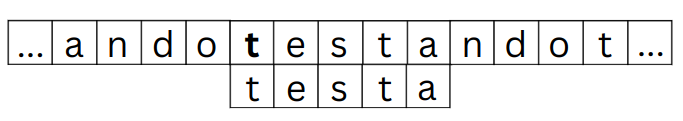
\includegraphics[width=0.6\linewidth]{Figuras/representacaoForcaBruta1.png}\\
                \caption{representação força bruta}
                \label{fig:ForcaBruta_1}
            \end{figure}

            \begin{figure}[h]
                \centering
                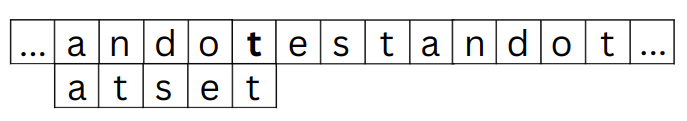
\includegraphics[width=0.6\linewidth]{Figuras/representacaoForcaBruta2.png}\\
                \caption{representação força bruta}
                \label{fig:ForcaBruta_2}
            \end{figure}

            Na figura 1, temos como texto a palavra 'testando' e como padrão 'testa'. Podemos observar que, ao usar 
            o 't' na primeira posição como nosso pivô, encontramos imediatamente o casamento, ao analisar a substring 
            gerada com 't' como a letra inicial. Nesse caso, nossa função retornaria imediatamente a posição de 't' 
            como a posição onde ocorreu o casamento. No caso em que o casamento não ocorre imediatamente, teríamos o 
            caso ilustrado na figura 2, onde continuamos com o mesmo pivô, mas consideramos o caractere como se fosse 
            a última letra de uma substring. Dessa forma, comparamos essa substring ao padrão invertido. Fazemos isso 
            para garantir a propriedade de que podemos ler a pedra tanto da esquerda para a direita quanto da direita 
            para a esquerda. No caso da figura 2, o casamento não ocorre, e nosso algoritmo avança escolhendo a 
            próxima posição do texto como um novo pivô e repetindo o processo.

            Caso não ocorra o casamento em nenhum momento, a função para ao analisar a última letra do texto como pivô, 
            retornando um valor negativo para indicar que não houve casamento.
            
        \subsection{Boyer-Moore-Horspool}
            O algoritmo de Boyer-Moore-Horspool é um dos algoritmos mais famosos para casamento de caracteres, sendo 
            uma simplificação feita por Horspool do algoritmo Boyer-Moore original. Assim como o força bruta, é bastante 
            simples de ser implementado e também eficiente.

            Em geral, o BMH funciona percorrendo o padrão da direita para a esquerda enquanto o compara com o texto, 
            de forma que, ao passarmos da primeira posição do padrão, teremos um casamento. No caso de um caractere do 
            padrão ser diferente de um caractere do texto, utilizamos uma tabela de deslocamentos que nos informa o 
            quanto podemos deslocar o padrão em relação ao texto. Essa tabela de deslocamentos é construída com base em 
            uma heurística que associa cada letra do nosso alfabeto a um número que nos diz o quanto podemos pular quando 
            houver uma colisão com essa letra. Em geral, toda letra do alfabeto que não está presente no padrão recebe 
            o tamanho do padrão como o número de deslocamento. Assim, especialmente para padrões que ocupam poucas letras 
            do alfabeto, temos um ganho significativo em termos de saltos e comparações em relação ao algoritmo de 
            força bruta. Mesmo em casos em que o padrão possui várias letras do alfabeto, ainda podemos obter ganhos.
            
            Para o nosso problema, continuaremos usando nosso TAD de lista circular para armazenar o texto e o padrão. 
            No entanto, para calcular nossa tabela de deslocamentos, passaremos o padrão como um vetor de caracteres 
            como parâmetro, para facilitar o acesso a cada uma de suas posições. A tabela de deslocamentos será armazenada 
            em um simples vetor de inteiros com 26 posições, em que cada posição N representa o deslocamento do caractere 
            "N + 97" da tabela ASCII, cobrindo assim todas as letras minúsculas do alfabeto latino. 
            Inicialmente, atribuiremos o tamanho do padrão a todas as posições do vetor. Em seguida, percorreremos o 
            padrão e, para cada uma de suas letras, atualizaremos a posição correspondente na tabela com o novo valor, que 
            é calculado usando a fórmula:
            \begin{displaymath}
               tabelaDeslocamentos[x] = min\{j \ tal \ que \ j = m \ | \ (1 \leq j < m \ \& \ padrao[m - j] = x)\}
            \end{displaymath}
            A função retornará a tabela de deslocamentos completa. 
            
            A partir disso, podemos finalmente verificar se existe um casamento, passando para nossa função BMH as listas 
            que armazenam o padrão e o texto, juntamente com a tabela de deslocamentos. Na função, seguiremos o princípio 
            do algoritmo BMH geral, mas teremos que adaptar alguns detalhes para atender às exigências do nosso problema.
            
            Primeiramente, como podemos ler o texto tanto da esquerda para a direita quanto da direita para a esquerda, 
            aplicaremos o algoritmo duas vezes, em cada direção. Para identificar um casamento da esquerda para a direita, 
            o algoritmo começa percorrendo o texto a partir da posição de índice igual ao tamanho do padrão, pois 
            compararemos o texto com o padrão da direita para a esquerda. Em seguida, iniciaremos o procedimento do BMH 
            normalmente. Percorreremos o padrão enquanto os caracteres forem iguais aos do texto e armazenaremos o índice 
            que indica a posição do padrão. Para verificar se houve casamento, basta observar se a posição é zero, ou seja, 
            se conseguimos percorrer o padrão até o final. Em caso afirmativo, não precisaremos continuar verificando por 
            novos padrões no sentido da esquerda para a direita no texto. Em caso negativo, continuaremos o procedimento 
            anterior, mas antes, verificaremos em qual posição do texto ocorreu a colisão e procuraremos na tabela de 
            deslocamentos o valor correspondente que nos dirá o quanto podemos avançar no texto.
            
            Depois disso, armazenaremos a posição do casamento, caso tenha ocorrido, e um valor negativo caso contrário. 
            Faremos isso porque precisaremos procurar a existência de casamentos olhando da perspectiva da direita para a 
            esquerda do texto. Faremos isso mesmo que tenhamos encontrado um casamento na primeira etapa, pois queremos 
            retornar a primeira posição onde ocorreu o casamento.
            
            Assim, prosseguimos com esta etapa, que é extremamente semelhante à primeira. De fato, só estaremos considerando 
            o texto como se estivéssemos lendo-o de trás para frente. Começaremos pela última posição e iremos para a 
            esquerda, em uma distância igual ao tamanho do padrão, de maneira semelhante à primeira fase. Em seguida, 
            seguiremos o BMH normalmente, mas, em vez de nos movermos pelo texto da direita para a esquerda, como na primeira 
            fase, nos moveremos da esquerda para a direita. No caso do padrão, continuaremos a nos mover normalmente, da 
            direita para a esquerda. Dessa forma, podemos simular que estamos lendo nossa lista invertida sem precisar inverter 
            a própria lista. Em seguida, verificaremos os casamentos e acessaremos a tabela de deslocamentos da mesma maneira 
            que na primeira fase, mas iremos percorrer o texto da direita para a esquerda, até esgotarmos as possibilidades de 
            novas comparações. Isso ocorre porque, na primeira fase, começamos da posição inicial do texto e nos movemos em 
            direção à posição final, e o primeiro casamento encontrado também é o de menor posição. Nessa segunda fase, isso 
            não é válido, pois estamos começando do final do texto e indo em direção ao início, o que significa que, em casos 
            de mais de um casamento, o primeiro a ser encontrado não é o de menor posição.
            
            Após realizar as duas fases, verificamos se alguma delas encontrou um casamento, e, caso ambas tenham encontrado, 
            retornamos a menor posição encontrada.
        
        
        \subsection{Shift-and}
            A terceira solução que utilizamos para resolver o problema é outro algoritmo famoso e bastante eficiente, o Shift-And. 
            Ele trabalha com o conceito de paralelismo de bits para simular um autômato que pesquisa pelo padrão no texto.

            O Shift-And utiliza uma tabela de máscara de bits, que mapeia cada letra do alfabeto usado. O número de bits para 
            cada letra é igual ao tamanho do padrão. Inicialmente, iniciamos a máscara de cada letra apenas com zeros. 
            Depois disso, para cada letra do alfabeto, colocamos 1 em cada posição em que a letra aparece no padrão. 
            Assim, caso uma letra não esteja no padrão, sua máscara será composta apenas de zeros. A partir dessa tabela, o 
            algoritmo inicia uma nova sequência de bits do tamanho do padrão e a preenche apenas com zeros. Em seguida, passamos 
            por cada letra do texto e utilizamos duas operações de bits: shift de um para a direita na sequência de bits inicializada 
            e operação AND entre essa sequência e a máscara correspondente à letra atual do texto. No caso de o último bit da 
            sequência ser um, temos um casamento de padrão.
            
            Um desafio ao implementar o Shift-And é o caso de o tamanho do padrão ser maior que o tamanho do texto, o que pode 
            acontecer em nosso problema. No entanto, em nosso caso, não precisaremos nos preocupar com isso, pois, com nosso TAD de 
            lista circular, podemos facilmente ir da última posição do texto para a primeira e vice-versa, o que nos permite ter 
            uma string infinita. Precisamos apenas definir uma condição de parada para nossas comparações com o texto, mas podemos 
            fazer isso observando que existe um momento em que começamos a fazer comparações repetidas com o texto, que é quando 
            passamos por todos os caracteres do texto mais o número de caracteres correspondente ao tamanho do padrão.
            
            Outra limitação do Shift-And ocorre devido a uma restrição no número de bits que uma variável inteira pode representar 
            na linguagem C. Basicamente, temos que o tipo 'unsigned long' possui 8 bytes, ou 64 bits. Assim, um padrão de entrada 
            com tamanho 100 não seria adequado ao programa, pois ele precisaria de 100 bits, o que ultrapassa o limite disponível no C. 
            Durante nosso desenvolvimento, conseguimos implementar o Shift-And de uma maneira na qual não usamos as operações 
            bit a bit nativas do C e suportamos uma entrada de qualquer tamanho. No entanto, esse algoritmo se mostrou muito ineficiente, 
            perdendo em desempenho até mesmo para o algoritmo de força bruta na maioria das entradas. Por esse motivo, decidimos 
            implementar um algoritmo com o limite de 64 bits, pois, pelo menos em entradas dentro desse limite, ele pode ser mais 
            eficiente, o que faz mais sentido para nossa análise de desempenho.
            
            Para implementar esse algoritmo, começamos criando a máscara de bits para cada letra de nosso alfabeto. Assim como a 
            tabela de deslocamentos usada no BMH, usamos um vetor para armazenar a máscara de cada letra. Com o auxílio das operações 
            bit a bit do C, conseguimos calcular com precisão a máscara de acordo com a explicação que demos sobre o algoritmo 
            anteriormente.
            
            O método Shift-And começa criando um conjunto de bits que armazena os prefixos que correspondem ao texto, a partir das 
            operações com a máscara das letras. Em seguida, de forma semelhante ao BMH, notamos que é necessário realizar duas pesquisas 
            no texto: uma caminhando da esquerda para a direita e outra caminhando da direita para a esquerda. Em ambos os sentidos, o 
            procedimento é o mesmo, mudando apenas a maneira como percorremos o texto. Ao iniciar a busca no texto, realizamos primeiro 
            a operação de shift de um bit para a direita em nosso vetor de bits e, em seguida, a operação AND com a máscara que 
            representa o caractere atual de nosso texto. Depois disso, verificamos se a última posição de nosso conjunto de bits é um, 
            ou seja, se o número é ímpar, e, em caso positivo, temos um casamento. Em caso negativo, avançamos para o próximo caractere 
            do texto. No caso em que pesquisamos da esquerda para a direita, como no BMH, podemos parar a busca assim que encontramos um 
            casamento. Já no caso em que pesquisamos da direita para a esquerda, devemos continuar até o final. Após executar ambos os 
            passos, verificamos qual foi a posição mais baixa em que ocorreu um casamento, se houver.

    %\newpage
    \section{ANÁLISE DE COMPLEXIDADE}
        Para compararmos as soluções e determinar qual é a melhor, é de extrema importância analisarmos suas complexidades, o que nos 
        ajudará a entender o comportamento do tempo de execução dos algoritmos em relação a diferentes entradas. Para isso, vamos focar 
        em determinar a complexidade de cada função em si, ignorando as partes de leitura e tratamento das entradas, pois são partes 
        comuns a todas as soluções.

        Para facilitar a explicação da complexidade, consideramos o tamanho do texto como sendo N e o tamanho do padrão como M.

        \subsection{Força bruta}
            Nossa solução com força bruta é a mais simples das três e não precisa de um processamento adicional, pois não necessita de 
            uma tabela de deslocamentos ou máscaras de bits como as outras.

            Para solucionar o problema, essa solução percorre cada letra do texto e, em cada letra, percorre cada letra do padrão duas 
            vezes, comparando-as com as do texto até chegar ao final e termos um casamento ou até as letras serem diferentes. Temos aí 
            uma vantagem em relação às outras duas soluções, pois em caso de encontrar o casamento, a função pode retornar imediatamente 
            a posição encontrada, pois o primeiro casamento achado será também o de menor posição.
            
            Assim, caso exista casamento nas primeiras posições, essa solução irá gerar poucas comparações.
            
            No caso de não existir casamento, esse algoritmo terá percorrido todas as N posições do texto, realizando, no pior caso, 
            um total de 2 * M comparações. Assim, a complexidade no pior caso é:
                \begin{displaymath}
                    fb(M, N) = (2 * M) + (2 * M) + ... + (2 * M) = 2 * M * N
                \end{displaymath}
            Note que o pior caso ocorre quando apenas a última letra do padrão é diferente do texto, como por exemplo, padrão = "aab" 
            e texto = "aaaaaaaaaa", o que é um caso raro, mas que pode sim acontecer.
            
            No caso médio, podemos esperar que, muitas vezes, serão realizadas apenas duas comparações na maioria das letras do texto, 
            isto é, a letra do texto ser diferente da primeira letra do padrão logo na primeira comparação. No caso em que isso sempre 
            acontece, teremos uma função linear, pois em cada posição teremos exatamente duas comparações:
                \begin{displaymath}
                    fb(M, N) = 2 + 2 + ... + 2 = 2 * N
                \end{displaymath}
            O caso médio tenderá a ser pior que o melhor caso, mas ainda não será tão ruim como o pior caso. Temos que:
                \begin{displaymath}
                    fb(M, N) = 26/25 * (1 - 1/(26^M)) * (N - M + 1) + O(1)
                \end{displaymath}
            Isso nos dá um resultado um pouco pior que linear. Por exemplo, para M = 7 e N = 15 e entradas aleatórias, teremos cerca de 
            12 comparações aproximadamente.

        \subsection{Boyer-Moore-Horspool}
            No caso do BMH, primeiro precisamos computar o processamento da tabela de deslocamentos. Temos que, primeiramente, o algoritmo 
            passa pelo vetor de deslocamentos 26 vezes, que é o tamanho de nosso alfabeto, e depois passa por ele novamente, dessa vez M 
            vezes, para colocar o valor de deslocamentos dos caracteres presentes no padrão. Assim, para calcular a tabela de deslocamentos, 
            temos:
                \begin{center}
                    tb(M) = M + O(1), pois as 26 operações têm tempo constante.
                \end{center}
            
            Depois, para fazer o cálculo de casamentos em si, executamos o BMH duas vezes, em ambas as direções que podemos andar pelo texto. 
            Na primeira execução, assim que o casamento é encontrado, não precisamos mais procurar por outro. Assim, no caso de termos um 
            casamento nas primeiras posições do texto, ele faz poucas comparações. Entretanto, na segunda fase, independentemente de haver 
            casamentos ou não, o algoritmo continua até esgotar as possibilidades de comparações únicas. Nessa segunda execução, no caso 
            especial de termos vários casamentos, o número de comparações seria alto.
            
            No geral, o BHM tem complexidade conhecida no pior caso de O(N * M), melhor caso de O(N / M) e caso esperado de O(N / M). 
            Como o executamos duas vezes, apenas multiplicamos sua função de complexidade por 2.

        \subsection{Shift-and}
            Para o Shift-And, também precisamos computar uma tabela, nesse caso, uma tabela com as máscaras de bits. Passamos por cada letra 
            do alfabeto, no nosso caso 26, e atualizamos a máscara de bits com base nos caracteres do padrão, assim, temos uma complexidade:
                \begin{center}
                    md(M) = M + O(1), pois o procedimento para inicializar a máscara é constante.
                \end{center}
        
            Para calcular os casamentos, o algoritmo também é executado duas vezes, uma para cada direção que podemos andar pelo texto. 
            Na primeira pesquisa, também podemos parar de procurar casamentos quando o primeiro for encontrado, e na segunda pesquisa também 
            temos que continuar até esgotar as opções de comparação. Assim, mais uma vez, quando encontramos um casamento nas primeiras 
            posições da primeira pesquisa, temos um grande ganho no número de comparações.
            
            O Shift-And irá executar, no geral, em O(N + M), pois dentro de um 'for' ele irá percorrer as N posições do texto, mais M posições 
            em relação ao tamanho do padrão, para garantir que passamos por todas as comparações possíveis. E em cada passo do 'for', serão 
            realizadas operações constantes, assim, nos dando uma complexidade de O(N + M).
        
        \subsection{Análise empírica da performance das soluções}
            Para demonstrar de maneira visual a performance dos algoritmos, realizamos diversos testes e comparamos os resultados de tempo 
            obtidos com as diretivas "gettimeofday" e "getrusage".

            Fizemos uma série de testes aleatórios, com padrões de tamanho menor que 64, para atender à limitação do Shift-And, e texto de 
            tamanho até 10.000, como foi especificado em nossa introdução. Nessas condições e com testes realizados em sequência, podemos 
            confirmar que todas as três soluções apresentam um comportamento muito próximo ao linear. Isso ocorre porque, em entradas 
            aleatórias, acontecem poucos casamentos, e é difícil encontrarmos o pior caso das soluções. Os gráficos abaixo mostram como cada 
            solução se comportou separadamente em um de nossos testes usando o 'gettimeofday':

            \begin{figure}[H]
                \centering
                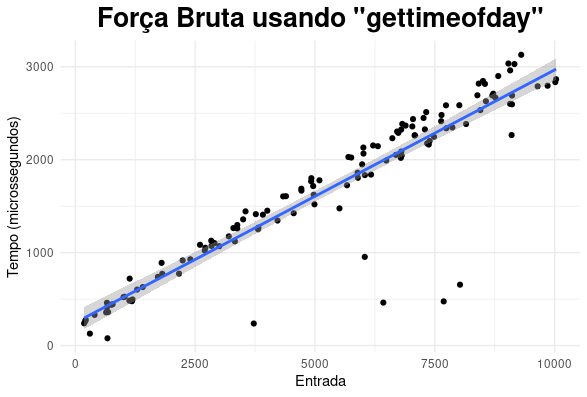
\includegraphics[width=0.6\linewidth]{Figuras/graficoFB.png}\\
                \caption{representação gráfico força bruta}
                \label{fig:GraficoFB}
            
                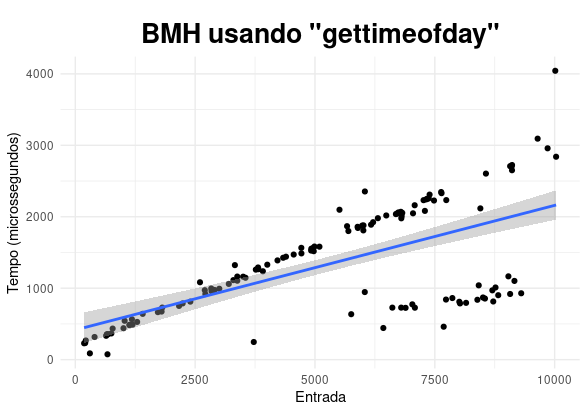
\includegraphics[width=0.6\linewidth]{Figuras/graficoBMH.png}\\
                \caption{representação gráfico Boyer-Moore-Horspool}
                \label{fig:GraficoBMH}
            
                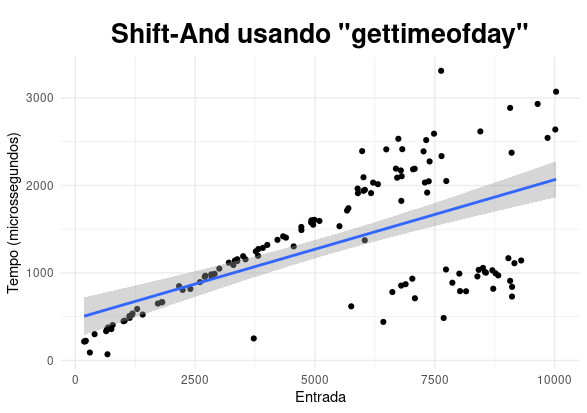
\includegraphics[width=0.6\linewidth]{Figuras/graficoSA.png}\\
                \caption{representação gráfico Shift-and}
                \label{fig:GraficoSA}
            \end{figure}
        
            Depois disso, realizamos outro teste, também com entradas aleatórias, e colocamos os resultados em um mesmo gráfico, para 
            podermos comparar melhor como as soluções se comportam entre si:
            
            \begin{figure}[H]
                \centering
                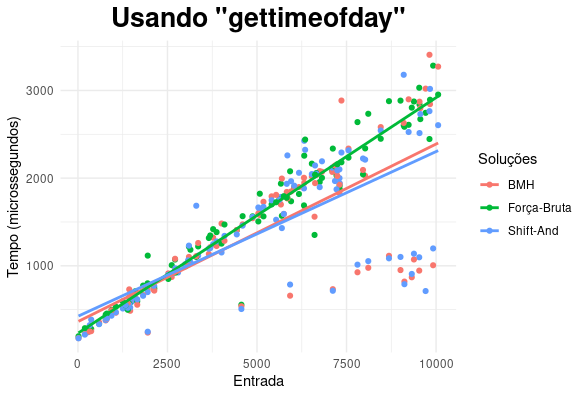
\includegraphics[width=0.6\linewidth]{Figuras/graficoGeralGTOD.png}\\
                \caption{representação gráfico gettimeofday}
                \label{fig:GraficoForcaBruta}
            
                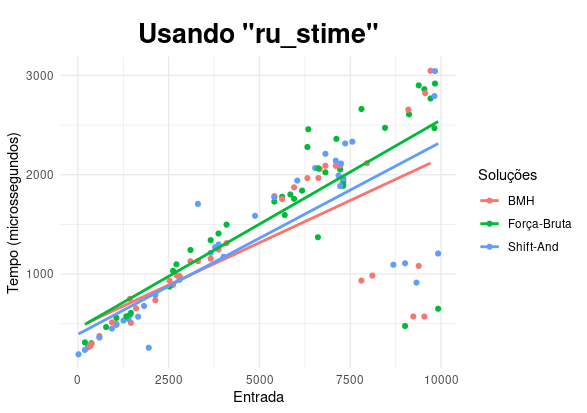
\includegraphics[width=0.6\linewidth]{Figuras/graficoGeralSistema.png}\\
                \caption{representação gráfico sistema}
                \label{fig:GraficoBMH}
            \end{figure}

    \section{CONCLUSÃO}
        Primeiramente, vale ressaltar a importância da análise cuidadosa das especificações iniciais do trabalho. Dadas as condições de tamanho 
        de nossas entradas, conseguimos construir três soluções em que todas conseguem resolver de maneira eficiente o problema proposto, com a 
        ressalva do Shift-And, que possui um limite de tamanho do padrão de 64.

        Com isso em mente, neste trabalho específico, verificamos que a performance do Shift-And com entradas aleatórias foi a melhor usando o 
        'gettimeofday' e a segunda melhor usando o 'getrusage', sempre com uma margem pequena em relação ao BMH. No entanto, consideramos que o 
        BMH é o algoritmo mais apropriado para a situação, devido às suas limitações de entrada e ao fato de não perder muito em desempenho em 
        relação ao Shift-And.
        
        Desta forma, concluímos ressaltando a importância de conhecer o comportamento assintótico de um algoritmo e de definir uma solução que 
        seja a melhor geral, ou seja, rápida e adequada às exigências iniciais. Cabe ao desenvolvedor pesquisar e concluir qual solução se 
        comportará melhor no problema dado.
	\newpage
    \nocite{Cormen2012}
    %\nocite{Backes2012}
	%\nocite{Backes2016}

	\addcontentsline{toc}{section}{REFERÊNCIAS}
	\bibliographystyle{apalike} % Estilo da bibliografia
	\bibliography{bibliografia} % Adiciona as referencias
\end{document}